%artigo científico sobre bel e decibel em abnt2


\documentclass[article, 11pt, oneside, a4paper, english, brazil, sumario=tradicional]{abntex2}
\usepackage{lmodern}			% Usa a fonte Latin Modern
\usepackage[T1]{fontenc}		% Selecao de codigos de fonte.
\usepackage[utf8]{inputenc}		% Codificacao do documento (conversão automática dos acentos)
\usepackage{indentfirst}		% Indenta o primeiro parágrafo de cada seção.
\usepackage{nomencl} 			% Lista de simbolos
\usepackage{color}				% Controle das cores
\usepackage{graphicx}			% Inclusão de gráficos
\usepackage{microtype} 			% para melhorias de justificação
\usepackage{amsmath}            % para as formulas matematicas ficarem bem visualmente

\usepackage{blindtext}
\usepackage[brazil]{babel}

% Pacotes de citações
\usepackage[brazilian,hyperpageref]{backref}	 % Paginas com as citações na bibl
\usepackage[alf]{abntex2cite}	% Citações padrão ABNT

% Configurações do pacote backref
% Usado sem a opção hyperpageref de backref
\renewcommand{\backrefpagesname}{Citado na(s) página(s):~}
% Texto padrão antes do número das páginas
\renewcommand{\backref}{}
% Define os textos da citação
\renewcommand*{\backrefalt}[4]{
	\ifcase #1 %
		Nenhuma citação no texto.%
	\or
		Citado na página #2.%
	\else
		Citado #1 vezes nas páginas #2.%
	\fi}%


% Informações de dados para CAPA e FOLHA DE ROSTO
\def \theforeigntitle{}
\titulo{Bel e Decibel}
\autor{Luís Henrique Martins Carvalho}
\local{Brasil}
\data{Maio, 2022}

% alterando o aspecto da cor azul
\definecolor{blue}{RGB}{41,5,195}
% informações do PDF
\makeatletter
\hypersetup{
     	%pagebackref=true,
		pdftitle={\@title}, 
		pdfauthor={\@author},
    	pdfsubject={Bel e Decibel},
	    pdfcreator={LaTeX with abnTeX2},
		pdfkeywords={abnt}{latex}{abntex}{abntex2}{atigo científico}, 
		colorlinks=true,       		% false: boxed links; true: colored links
    	linkcolor=blue,          	% color of internal links
    	citecolor=blue,        		% color of links to bibliography
    	filecolor=magenta,      		% color of file links
		urlcolor=blue,
		bookmarksdepth=4
}
\makeatother

% compila o indice
\makeindex

% Altera as margens padrões
\setlrmarginsandblock{3cm}{3cm}{*}
\setulmarginsandblock{3cm}{3cm}{*}
\checkandfixthelayout

% Espaçamentos entre linhas e parágrafos 
% O tamanho do parágrafo é dado por:
\setlength{\parindent}{1.3cm}
% Controle do espaçamento entre um parágrafo e outro:
\setlength{\parskip}{0.2cm}  % tente também \onelineskip
% Espaçamento simples
\SingleSpacing

% Definição de cores
\definecolor{codegreen}{rgb}{0,0.6,0}
\definecolor{codegray}{rgb}{0.5,0.5,0.5}
\definecolor{codepurple}{rgb}{0.58,0,0.82}
\definecolor{backcolour}{rgb}{0.97,0.97,0.95}

\begin{document}
    % Retira espaço extra obsoleto entre as frases.
    \frenchspacing 
    \maketitle
    \begin{resumoumacoluna}

        Foi inventado por engenheiros do Bell Labs para quantificar a redução no nível
    acústico sobre um cabo telefônico padrão com 1 milha de comprimento. Decibel (dB) é uma unidade inventada para medir a intensidade do som. Ela é uma razão entre valores, com um valor de referência. Como a
    intensidade absoluta dos sons varia em uma escala muito grande, a unidade é definida em termos de
    uma escala logarítmica.

 \vspace{\onelineskip}
 
 \noindent
 \textbf{Palavras-chaves}: Decibel. Bel. Som. Unidade. Logaritmo.
\end{resumoumacoluna}

    \section*{Introdução}
    \addcontentsline{toc}{section}{Introdução}
        O decibel (dB) é uma medida da razão entre duas quantidades,
    sendo usado para uma grande variedade de medições em acústica,
    física, eletrônica e telecomunicações. Por ser uma razão entre duas
    quantidades iguais o decibel é uma unidade de medida adimensional
    semelhante a percentagem. O dB usa o logaritmo decimal (log10) para
    realizar a compressão de escala. Um exemplo típico de uso do dB é na
    medição do ganho/perda de potência em um sistema. Além do uso do
    dB como medida relativa, também existem outras aplicações na
    medidas de valores absolutos tais como potência e tensão entre outros
    (dBm, dBV, dBu). O emprego da subunidade dB é para facilitar o seu
    uso diário (Um decibel (dB) corresponde a um décimo de bel (B)). \cite{apostila_ifsc}

    \section{Definição}
    O bel (símbolo: B) é uma unidade de medida adimensional, que compara a intensidade de um sinal a um nível de referência. Recebe este nome em homenagem ao físico Alexander Graham Bell. O cálculo é mais frequente em decibel. \cite{wiki:xxx}
    A unidade bel é usada para caracterizar o logaritmo decimal da razão entre duas quantidades similares de energia ou potência $P_1$ e $P_2$:
    \begin{equation*}
        Q_{(P)} = \log \frac{P_{1}}{P_{2}} \mathrm{B} = 10 \log \frac{P_{1}}{P_{2}} \mathrm{dB}
    \end{equation*}

    Para ${Q_{(P)}}$, por exemplo, o valor 1 B resulta quando a razão de potência é ${\frac{P_{1}}{P_{2}}} = 10 $. O decibel, por sua vez, é formado com o acréscimo do prefixo d (deci): 
    \begin{equation*}
        1 \mathrm {dB} = \frac{1}{10} \mathrm{B}
    \end{equation*}
    
    O decibel pode expressar uma alteração no valor (por exemplo, +1 dB ou $-1$ dB) ou um valor absoluto. No último caso, o valor numérico expressa a proporção de um valor para um valor de referência fixo; quando usado dessa forma, o símbolo da unidade geralmente é sufixado com códigos de letras que indicam o valor de referência. Por exemplo, para o valor de referência de 1 volt, um sufixo comum é "V" (por exemplo, "20 dBV")

    As normas ISO 80000-8 e 60027-3 descrevem as definições para grandezas físicas e quantidades, entre as quais o decibel. De acordo com essas definições, o decibel (1 dB) é uma décima parte do bel. O bel (B), por sua vez, é definido como 0,5 log(10) neper: 1 B = 0,5 log(10) Np. Por sua vez, o neper é definido como a mudança em nível de uma quantidade de potência-raiz quando a quantidade de potência-raiz muda por um fator de e, ou seja, 1 Np = ln(e) = 1, relacionando, assim, todas as unidades como o logaritmo natural não-dimensional das relações potência-raiz-quantidade, 1 dB = 0.115 13… Np = 0.115 13…. Finalmente, o nível de uma quantidade é o logaritmo da razão entre o valor dessa quantidade e um valor de referência do mesmo tipo de quantidade. Essas definições permitem estabelecer as seguintes igualdades:
    
    \begin{equation*}
        1 \mathrm{dB} = 0,1 \mathrm{B}
    \end{equation*}
    \begin{equation*}
        {\displaystyle 1{\text{ B}}={\frac {1}{2}}\log _{e}\left({\frac {Q}{Q_{0}}}\right)\,{\text{Np}}=10\log _{10}\left({\frac {Q}{Q_{0}}}\right) {\text{dB}}}
    \end{equation*}
    
    onde $Q$ é a quantidade medida e $Q_0$ o valor de referência.\\
    
    Portanto, o bel representa o logaritmo de uma razão entre duas grandezas de potência de 10:1, ou o logaritmo de uma proporção entre duas grandezas de potência-raiz de $\sqrt{10:1}$. Logo, duas quantidades cujos níveis diferem em um decibel têm uma relação de potência de $10^{1/10}$, o que corresponde aproximadamente a 1,25893, e uma amplitude (quantidade potência-raiz) cujo rácio é $10^{1/20}$ (aproximadamente 1,12202).
    
        Como a potência é proporcional ao quadrado da tensão dividida pela
    resistência do circuito, temos, aplicando as propriedades dos logaritmos (o log.
    do quadrado de n é duas vezes o log. de n) :
    
    \begin{equation*}
        Q_{(dB)} = 20 \log \frac{V_1}{V_2} + 10 \log \frac{R_2}{R_1}
    \end{equation*}
    
    ou ainda, na mesma resistência :
    
    \begin{equation*}
        Q_{(dB)} = 20 \log \frac{V_1}{V_2}
    \end{equation*}
    
        Para ganhos por ex., $P_2$ é a potência de entrada e $P_1$ a potência de saída do
    circuito.
        Para atenuações, $P_1$ é a potência de entrada e $P_2$ a potência de saída.
    Atenuação é o inverso do ganho (em unidades lineares) e é igual ao ganho em
    dB com sinal trocado.
    
    \begin{table}[ht]
\centering
\begin{tabular}{|c|c|c|}
\hline
$Q_{(db)}$ & $P_1$/$P_2$ & $V_1$/$V_2$\\
\hline
120 & $10^{12}$ & 1000000\\
90 & $10^{9}$ & 31600\\
60 & $10^{6}$ & 1000\\
30 & $10^{3}$ & 31.6000\\
20 & $10^{2}$ & 10\\
10 & $10^{1}$ & 3.1600\\
6 & 4.00 & 2\\
3 & 2.00 & 1.4140\\
0 & 1.00 & 1\\
-3 & 0.50 & 0.7070\\
-6 & 0.25 & 0.5000\\
-10 & $10^{-1}$ & 0.3160\\
-20 & $10^{-2}$ & 0.1000\\
-30 & $10^{-3}$ & 0.0316\\
-60 & $10^{-6}$ & 0.0010\\
-120 & $10^{-12}$ & $10^{-6}$\\
\hline
\end{tabular}
\caption{valores típicos \cite{bel1}}
\end{table}

    
    Observe que 0 dB (zero dB) equivale a uma relação de 1, e 3 dB equivale a uma relação de 2 ( em potência), e 10 dB por acaso equivale a uma relação de 10, ou seja, +3 dB equivale a multiplicar por 2, +10 dB equivale a multiplicar por 10, -3 dB equivale a dividir por 2, -10 dB equivale a dividir por 10.
    
    

    \section{Valores absolutos e valores relativos}
    O decibel é o resultado de uma relação logaritma entre a potência que entra em um sistema e a potência que sai do mesmo. Se o valor resultante for positivo, significa que o sinal de saída é maior que o sinal de entrada, o que representa um ganho no sistema. Se o sinal de saída for negativo, significa que o sinal de entrada é maior que o sinal de saída, o que representa uma perda no sistema. \cite{embarcados}
    
    \begin{equation*}
        Ganho_{dB} = 10 \cdot \log (\frac{P_{saida}}{P_{entrada}})
    \end{equation*}
    
    O cálculo de ganho ou perda de um sistema em decibel terá como resposta um valor absoluto. Dizer que um amplificador tem ganho de 30 dB significa dizer que ele aumenta uma potência de entrada em 1000 vezes. Uma linha de transmissão que tem uma perda de 20 dB, atenua a potência de entrada em 100 vezes.
    
    Perceba que o resultado obtido (1000 vezes) independe da unidade de medida utilizada (watts). Usando as propriedades matemáticas dos logaritmos é fácil perceber que para saber em quantas vezes é o ganho ou perda de um sistema para um valor em dB.

    \begin{equation*}
        X_{(vezes)} = 10^{(\frac{dB}{10})}
    \end{equation*}
    
    \begin{figure}[ht]
        \centering
        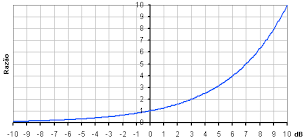
\includegraphics{db_razaop.png}
        \caption{Relação dB x Razão de potência. (Flávio Archangelo, 2011)}
    \end{figure}
    
    \newpage
    Na eletrônica pode ser conveniente relacionar o decibel a uma referência. O valor a ser encontrado será relativo à unidade de medida usada como referência. Um exemplo é a unidade dBm. Ela representa a medida de potências em relação a 1 mW. Assim, pode-se converter valores de watts para dBm. Esta medida não representa o ganho ou a perda de um sistema, e sim um valor de potência que é emitido ou recebido por um equipamento.
    
    \begin{equation*}
        \text{Potência}_{(dBm)} = 10 \cdot \log (\frac{P_{W}}{0,001W})
    \end{equation*}

    \section{Decibel na medida física do som}
    O som é uma oscilação na pressão do ar (ou de outro meio elástico) capaz de ser percebida pelo ouvido humano. O número de oscilações da pressão do ar por unidade de tempo definem sua frequência, enquanto que a magnitude da pressão média define a potência e a intensidade sonora. A frequência é expressa em hertz (ou ciclos/segundo) e a pressão em pascal (ou newtons/$m^2$), enquanto que a potência é a energia emitida pela fonte sonora por unidade de tempo, expressa em joules/s ou W (estamos usando unidades do Sistema Internacional). A intensidade sonora pode ser definida como potência por unidade de área, expressa em watt/m2. Essas escalas para medida de pressão, potência e intensidade das ondas sonoras são escalas lineares.

    Contudo, a pressão, a potência e a intensidade dos sons captados pelo ouvido humano cobrem uma ampla faixa de variação.Por exemplo, um murmúrio irradia uma potência de 0,000 000 001 watt ($10^{-9} W$) enquanto que o grito de uma pessoa comum tem uma potência sonora de cerca de 0,001 watt; uma orquestra sinfônica chega a produzir 10 watts enquanto que um avião a jato emite 100 000 watts de potência ao decolar. Sendo assim, uma escala logarítmica, como o decibel, é mais adequada para medida dessas grandezas físicas. Por este motivo, são usadas as seguintes escalas logarítmicas:
    
    \subsection{Nível de Pressão Sonora}
        ${db_{SPL}} = 20 \log (P_{ef} / P_{o})$
        
        $P_{ef} = \text{valor eficaz da pressão sonora}$
        
        $P_{o} = 2 \times 10^{-5} N / m^{2}$
    
    \subsection{Nível de Intensidade Sonora}
        $dB_{IL} = 10 \log(I/I_{o})$

        $I = \text{intensidade acústica} \, I_{o} = 10^{-12} W / m^{2}$
    
    \subsection{Nível de Potência Sonora}
        $dB_{PWL} = 10 \log (W/W_{o})$

        $W = \text{potência acústica}$

        $W_{o} = 10^{-12} W $
        
    \subsection*{}
    Os valores de referência, Po, Io e Wo, correspondem aos limiares (ou umbrais) de percepção do ouvido humano. Note que o dB no umbral é zero. Nas expressões acima, SPL = sound pressure level (nível de pressão sonora); IL = (sound) intensity level (nível de intensidade sonora); PWL = (sound) power level (nível de potência sonora). 

\begin{table}[ht]
\centering
\begin{tabular}{|c|c|c|}
\hline
Fontes de ruído & Intensidade (Watt/$m^{2}$) & dB\\
\hline
limite da dor & $10^{2}$ & 140\\
jato & $10^{0}$ & 120\\
britadeira & $10^{-2}$ & 100\\
via movimentada & $10^{-4}$ & 80\\
barulho de escritório & $10^{-6}$ & 60\\
escritório privado residencia & $10^{-8}$ & 40\\
estúdio de rádio operando & $10^{-10}$ & 20\\
limite da audição & $10^{-12}$ & 0\\
\hline
\end{tabular}
\caption{Níveis sonoros}
\end{table}


    \section{Outras escalas logarítmicas}
O neper é uma unidade similar que usa o logaritmo natural. A escala
Richter também usa números expressos em bels. Na espectrometria e
na óptica as unidades de absorbância são equivalentes a $ - 1 $ B. Na
astronomia a magnitude aparente que mede o brilho das estrelas
também é uma unidade logarítmica, uma vez que da mesma forma que
o ouvido responde de modo logarítmico a potencia acústica, o olho
também responde de modo logarítmico a intensidade luminosa.

    \section{Considerações finais}
    As vantagens do uso do decibel são

    É mais conveniente somar os valores em decibels em estágios sucessivos de um sistema do que multiplicar os seus fatores de multiplicação.
    Faixas muito grandes de razões de valores podem ser expressas em decibels em uma faixa bastante moderada, possibilitando uma melhor visualização dos valores grandes.
    Na acústica o decibel usado como uma escala logarítmica da razão de intensidade sonora, se ajusta melhor a intensidade percebida pelo ouvido humano, pois o aumento do nível de intensidade em decibels corresponde aproximadamente ao aumento percebido em qualquer intensidade, fato conhecido com a Lei de potências de Stevens. Por exemplo, um humano percebe um aumento de 90 dB para 95 dB como sendo o mesmo que um aumento de 20 dB para 25 dB.

    
    \bibliography{referencias}
    
    \section*{Código fonte das tabelas}
        \lstinputlisting[
                title=\lstname,
                label={lst:listagem-c},
                language=C,
                backgroundcolor=\color{backcolour},   
                commentstyle=\color{codegreen},
                keywordstyle=\color{magenta},
                numberstyle=\tiny\color{codegray},
                stringstyle=\color{codepurple},
                basicstyle=\ttfamily\footnotesize,
                breakatwhitespace=false,
                breaklines=true,
                keepspaces=true,
                numbers=left,
                numbersep=5pt,
                showspaces=false,
                showstringspaces=false,
                showtabs=false,
                tabsize=4,
            ]{main.c}
\end{document}

